%*******************************************************************************
%*********************************** First Chapter *****************************
%*******************************************************************************

\chapter{GIỚI THIỆU}  %Title of the First Chapter

\ifpdf
    \graphicspath{{Chapter1/Figs/Raster/}{Chapter1/Figs/PDF/}{Chapter1/Figs/}}
\else
    \graphicspath{{Chapter1/Figs/Vector/}{Chapter1/Figs/}}
\fi


%********************************** %First Section  **************************************
\section{Ý tưởng và tính cấp thiết của đề tài}\label{section1.1}

Ngày nay, bài toán giao thông vẫn đang là bài toán hóc búa vẫn chưa được giải quyết được ở Việt Nam và nhiều nước đang phát triển. Tình trạng kẹt xe, ùn tắc kéo dài gây ra sự chậm trễ trong công việc, hơn nữa còn  gây gia tăng ô nhiễm môi trường, giảm chất lượng môi trường sống. Một trong những khó khăn làm bài toán giao thông khó giải quyết đó chính là không có đầy đủ dữ liệu cần thiết. Chúng ta không thể giải bài toán nếu không có đủ dữ kiện, cũng như giải quyết kẹt xe ta cần phải có dữ liệu về lưu lượng giao thông.

Vì yếu tố trên, dự án Smart Traffic được hình thành và phát triển theo hướng IoT với mục đích thu thập dữ liệu về các yếu tố môi trường (nồng độ CO, nhiệt độ, độ ẩm, nồng độ bụi, độ ồn…) và xác định mối tương quan giữa lưu lượng giao thông với môi trường xung quanh khu vực đó. Từ đó ta có thể có được 1 phần dữ liệu cần thiết về tình trạng các con đường theo thời gian thực, cũng như có được lịch sử và dùng dữ liệu ấy để phát triển dự đoán tình trạng giao thông tiếp theo.

\begin{figure}[H] 
\centering    
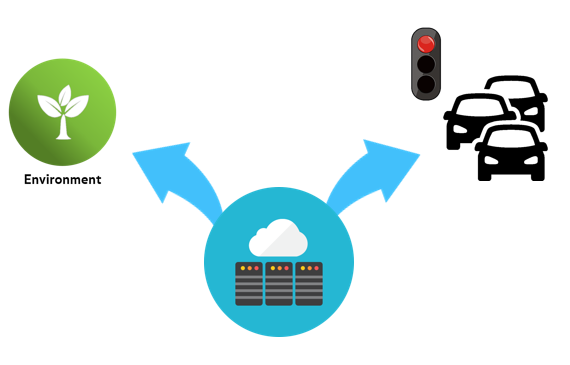
\includegraphics[width=1.0\textwidth]{pic1}
\caption[Mo hinh IoT ]{Mo ta tam hinh Mo hinh IoT}
\label{fig:pic1}
\end{figure}

Những dữ liệu đó có thể được phân tích và xử lý, đưa ra những kết luận về tình trạng lưu thông trên đoạn đường đó, về sự thay đổi môi trường tại 1 khu vực ở những khoảng thời gian khác nhau. Và những dữ liệu này có thể ứng dụng cho bất động sản, môi trường và nghiên cứu. Do đó đề tài mang tính thiết thực và ứng dụng cao và được lựa chọn để làm Thực tập tốt nghiệp và có thể lên Luận văn tốt nghiệp.




\section{Mục tiêu và nhiệm vụ của đề tài} %Section - 1.1 
\label{section1.2}
\subsection{Mục tiêu đề tài}
\begin{itemize}
\item[-]Tìm hiểu về khí thải xe máy và ô tô.

\item[-]Hiện thực mạch cảm biến để thu thập khí thải.

\item[-]Khảo sát và đo khí thải thực tế tại một số điểm thường xuyên xảy ra kẹt xe trên địa bàn thành phố.

\item[-]Tổng hợp các số liệu thu thập và các yếu tố môi trường khác (nhiệt độ, độ ẩm, …) để đề xuất mô hình để hướng đến phát triển hệ thống cảnh báo kẹt xe dựa vào tình trạng ô nhiễm không khí.




\end{itemize}

\subsection{Nhiệm vụ đề tài}
Phân chia công việc tại đây!!!! Sony, Tùng, Cường làm nhừng gì, vẽ giản đồ gantt.

\section{Cấu trúc báo cáo} %Section - 1.1 
